\documentclass{article}

% Language setting
% Replace `english' with e.g. `spanish' to change the document language
\usepackage[french]{babel}
\usepackage[fleqn]{amsmath} % Aligner les équations à gauche


% Set page size and margins
% Replace `letterpaper' with`a4paper' for UK/EU standard size
\usepackage[letterpaper,top=2cm,bottom=2cm,left=3cm,right=3cm,marginparwidth=1.75cm]{geometry}

% Useful packages

\usepackage{amsmath}
\usepackage{graphicx}
\usepackage{subcaption}
\usepackage[colorlinks=true, allcolors=blue]{hyperref}

\title{TD 9}
\author{IPESUP - PC }
\date{17/01/24}

\begin{document}
\maketitle



\section{Jet d'eau sur une plaque}

On suspend une plaque rectangulaire de dimensions $l \times L$ par une extrémité, puis on dirige sur la plaque un jet d'eau horizontal d'épaisseur $e$ à une vitesse $\vec{v_0}$, et à une distance $h$ du point d'accroche.
Au contact de la plaque, le jet d'eau se scinde en deux jets d'épaisseur $e'$ et $e''$. 
Sous l'impact du jet, la plaque s'incline d'un angle $\alpha$ par rapport à la verticale.
On néglige l'influence de la gravité sur le jet

\begin{enumerate}
  \item En appliquant le TMC, calculer $\alpha$.
  \item Calculer la force exercée par l'eau sur la plaque
  \item Calculer $e$ et $e''$. 
\end{enumerate}

\begin{figure}[h]
  \centering
  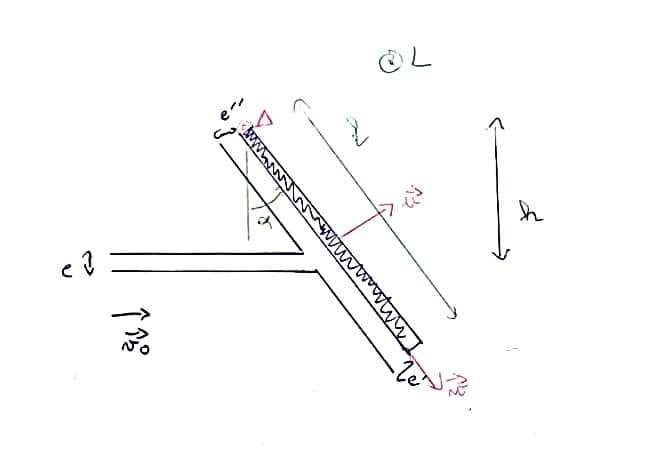
\includegraphics[width=0.5\textwidth]{schéma_plaque.jpg}
  \caption{Schéma du jet d'eau}
  \label{fig:jet}
\end{figure}
\section{Manomètre}

Considérons un écoulement avec un débit $Q$, à travers une contraction. Les pressions
à l’amont et à l’aval de la contraction sont mesurées à l’aide d’un manomètre (voir figure
) contenant de l’huile de masse volumique $\rho_e < \rho_h $. Les sections amont et aval
sont notées respectivement $A1$ et $A2$. Déterminer la hauteur $h$ donnée par le manomètre

\begin{figure}[h]
  \centering
  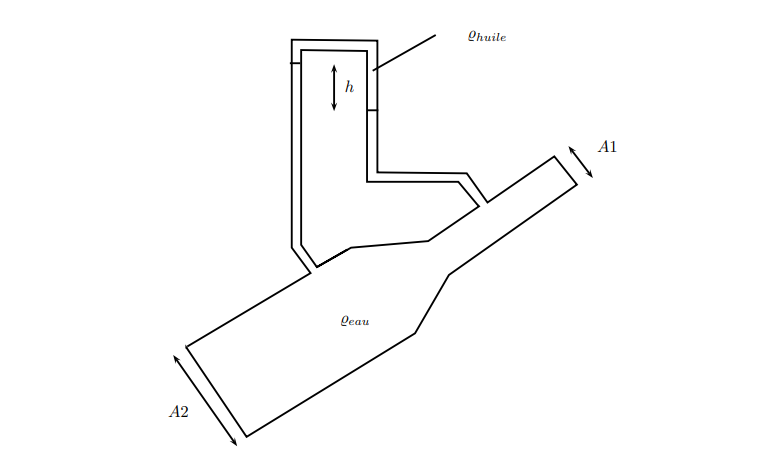
\includegraphics[width=0.5\textwidth]{manomètre.png}
  \caption{Manomètre}
  \label{fig:manometre}


\end{figure}
\newpage

\section{Vortex de Rankine:}

On considère un grand récipient rempli d'eau dans lequel on créé un tourbillon de vecteur de vorticité $\vec{\Omega} = \omega \vec{u_z}$, dans un cylindre de rayon $a$.
La vorticité est nulle pour $r>a$. 
On considèrre que le récipient est suffisament grand pour que le fluide occupe tout le demi-espace $z<0$.
\begin{enumerate}
  \item Déterminer le champ de pression on tout point du fluide. 
  \item Quelle est la forme de la surface libre ? 


\end{enumerate}

\section{Centrale PC 1 2023}

On traitera les questions 27 à 33. 

\end{document}

